\documentclass{ltjsbook}
\usepackage{docmute} 
\usepackage{../../myStyle} 

\begin{document}
\chapter{構造方程式モデリング}
\label{L09_SEM}

最後に\keyterm{構造方程式モデリング}{こうぞうほうていしきもでりんぐ}{Structural Equation Modeling, SEM}について説明していきます\footnote{この手法は別名\keytermL{共分散構造分析}{きょうぶんさんこうぞうぶんせき}という名前でも呼ばれています。書籍や論文を検索する時は，こちらの名称もキーワードにしてみてください。}。この手法はこれまで学んできた因子分析や回帰分析を統合したもので，分散共分散行列に方程式を作り込んでいくものです。我々が調査で得たデータから得られる情報は，分散共分散行列がすべてですから，その変数間関係を細かく作り込んでいき，行列の隅々まで考え尽くすという意味で，究極の手法といえるでしょう。実際，SEMは因子分析や回帰分析の他にも，多くのモデルをその下位モデルとして包含します。言い換えれば，SEMが登場する前に考えられてきたさまざまなモデルが，SEMの枠組みで理解・表現できるようになりました。であれば，この究極の技さえ知っておけば，非常に広範囲に拡張できるわけですから，こんなに便利なことはありません。

構造方程式モデリングについても，データが作る行列の世界をイメージすると理解しやすくなります。
\section{構造方程式モデルによる未知数の推定}
\subsection{準備}
ここまでの話は，特に推測統計学的な説明を含んでいませんでした。しかし心理学では一般に標本と母集団を区別し，母集団での一般化した議論を展開していきますし，構造方程式モデリングでも基本的には母数の話をしたいところですので，少し準備をしておきます。

これまでの平均，分散は次のように定義してきました。
\[ \bar{x} = \frac{1}{n}\sum_i^n x_i \]
\[ s_x^2 = \frac{1}{n} \sum_i^n (x_i - \bar{x})^2 \]
これらはあくまでも標本の統計量であって，母数の推定値とするためには分散を
\[ \hat{\sigma^2} = \frac{1}{n-1}\sum_i^n  (x_i - \bar{x})^2 \]
で計算します。

また，推定したい母集団の状態は，基本的に\keytermL{確率分布}{かくりつぶんぷ}であると考えますので，確率についての考え方も少し取り入れる必要があります。確率変数の平均は\keytermL{期待値}{きたいち}と呼ばれ，確率変数Xの期待値は
\[ E[X] = \sum p_k x_k \]
で定義します。ここで$p_k$は変数Xが$x_k$の値になる確率であり，確率と実現値の積和で表されるものです。確率変数の分散は，次のようになります。
\[ V[X] = \sum p_k(x_k - E[X])^2 = E[(X-E[X])^2] \]

こうした平均・分散の表現の違いはありますが，行列計算も同様に考えることができます。たとえばデータの平均ベクトル
\[ \bar{\bm{x}} = \frac{1}{n}\bm{X}'\bm{1} \]
についても，
\[ E[\bm{x}] = (E[x_1],E[x_2],\cdots,E[x_m]) =(\mu_1,\mu_2,\cdots,\mu_m)' = \bm{\mu}' \]
のように表現しますし，母集団における分散共分散行列も，
\[ \bm{\Sigma} = E[(\bm{x}-\bm{\mu})(\bm{x}-\bm{\mu})'] = E[\bm{v}\bm{v}'] \]
のように表します。母集団における相関行列は，
\[ \bm{\Sigma}_r = E[\bm{z}\bm{z}']\]
など，平均・分散の表記が少し変わっただけ，と思っていただければ結構です。

\subsection{識別の問題}

さて，たとえば回帰分析モデルは，次のような方程式で表せるのでした。

\[ y = b_0 + b_1 x + e \]

またたとえば，因子分析モデルも，同様に次のような方程式で表せでしょう。

\[ \left \{
    \begin{array}{rcl}
        x_1 & = & \lambda_1 f + e_1 \\
        x_2 & = & \lambda_2 f + e_2 \\
        x_3 & = & \lambda_3 f + e_3 \\
    \end{array}
    \right .
\]

ここで$f$は因子得点，$\lambda_j$は因子負荷量，あるいはパス係数を表しています。

この因子分析モデルを例に，この方程式をどのように解くかをみていきましょう。誤差の平均は0，という特徴は$\bm{E} \left[ \bm{e} \right] = \bm{0}$と表すことができます。因子得点も標準化されていると仮定しますので，$\bm{E} \left[ \bm{f}\right] = \bm{0}$ですね。

つぎにベクトルの分散を関数$\bm{V}$で表すとします。データベクトル$\bm{x}$が平均0，あるいは平均偏差，あるいは標準化されていると考えると，$\bm{V} \left [ \bm{x} \right] =\bm{E} \left[ ( \bm{x} - \bm{E}\left[ \bm{x} \right] )^2 \right ] = \bm{E} \left [ \bm{xx}'\right]$は分散共分散行列$\bm{\Sigma}$だと考えることができます。また因子は標準化されているので$\bm{V}\left [ \bm{f} \right ] = 1$，誤差同士は相関しないものの，誤差には分散がありますので$\bm{V}\left[ \bm{e} \right]=\bm{E} \left[ \bm{ee}'\right] = \Psi$とします。ここで$\Psi$は対角に誤差分散が入った対角行列です。

さて，さきほどの3項目1因子モデルを行列で表現してみましょう。各要素を次のようにベクトルでまとめて表現します。
\[ \bm{x} = \begin{pmatrix} x_1\\x_2\\x_3 \end{pmatrix}, \bm{\Lambda} = \begin{pmatrix} \lambda_1\\ \lambda_2 \\ \lambda_3 \end{pmatrix}, \bm{e} = \begin{pmatrix} e_1 \\ e_2 \\ e_3 \end{pmatrix} \]
すると式は次のようにあっさり表現できます。
\[ \bm{x} = \bm{\Lambda} \bm{f} + \bm{e} \]
ここからデータの分散共分散行列$\bm{\Sigma}$を考えてみましょう。

\begin{eqnarray*}
    \bm{V}\left[ \bm{x} \right] &=& \bm{E}\left[ \bm{xx'}\right]\\
    &=& \bm{E}\left[ (\bm{\Lambda f}+\bm{e}) (\bm{\Lambda f}+\bm{e})' \right] \\
    &=& \bm{E}\left[ (\bm{\Lambda f}+\bm{e}) (\bm{f \Lambda' }+\bm{e'}) \right] \\
    &=& \bm{E}\left[ \bm{ \Lambda f^2 \Lambda' + \Lambda f e'  + ef\Lambda’ + ee' } \right] \\
    &=& \bm{\Lambda \Lambda'} + \Psi \\
\end{eqnarray*}

これをエレメントワイズで書き出すと次のようになります。
\begin{eqnarray*}
    \begin{pmatrix} s_1^2 & s_1s_2 & s_1s_3 \\
                      & s_2^2  & s_2s_3 \\
                      &        & s_3^2\end{pmatrix}
    &=& \begin{pmatrix} \lambda_1\\ \lambda_2 \\ \lambda_3 \end{pmatrix}\begin{pmatrix} \lambda_1 & \lambda_2 & \lambda_3 \end{pmatrix} + \begin{pmatrix} \sigma_1^2 & & \\ & \sigma_2^2 & \\ & & \sigma_3^2 \end{pmatrix} \\
    &=& \begin{pmatrix} \lambda_11^2 + \sigma_1^2 & \lambda_1\lambda_2       & \lambda_1 \lambda_3      \\
                                          & \lambda_2^2 + \sigma_2^2 & \lambda_2 \lambda_3      \\
                                          &                          & \lambda_3^2 + \sigma_3^2\end{pmatrix}
\end{eqnarray*}

この式の左辺はデータから計算された分散共分散行列，右辺はモデルから計算された分散共分散行列です。行列の下三角が消えているのは対称行列で同じ情報が入るからで，データからオリジナルに得られるのは3つの分散($s_1^2,s_2^2,s_3^2$)と3つの共分散($s_1s_2,s_1s_3,s_2s_3$)の情報になります。一方右辺での未知数はパス係数(因子負荷量)の$\lambda_1,\lambda_2,\lambda_3$と誤差分散$\sigma_1^2,\sigma_2^2,\sigma_3^2$ということになります。未知数の数と既知数の数が同じなので，この方程式は解けます。とくに，未知数と既知数の数が一致しているので，\keyterm{丁度識別}{ちょうどしきべつ}{just identification}，あるいは単に\keyterm{識別可能}{しきべつかのう}{identifiable}といいます。

分散共分散行列で提供される情報の増え方に比べて，モデルの未知数の増え方は小さいので，一般的なSEMのモデルのほとんどは\keytermL{過剰識別}{かじょうしきべつ}になります。つまりいくつかの答えがあり得る，ということになるので，その時は尤度が最も高くなるように，といった基準を加えて答えを一意に定めます。逆に未知数の方が多い場合\keytermL{識別不可能}{しきべつふかのう}(解が求められない)ということになり，その場合はどこかのパラメータを値として入れてやる(\keytermL{制約}{せいやく}をかける，といいます)必要があります。

\subsection{複雑なモデルの場合}

では次に，図\ref{fig::12_05}のような複雑なモデルでも方程式で表せることを示しましょう。
\begin{figure}[h]
    \begin{center}
        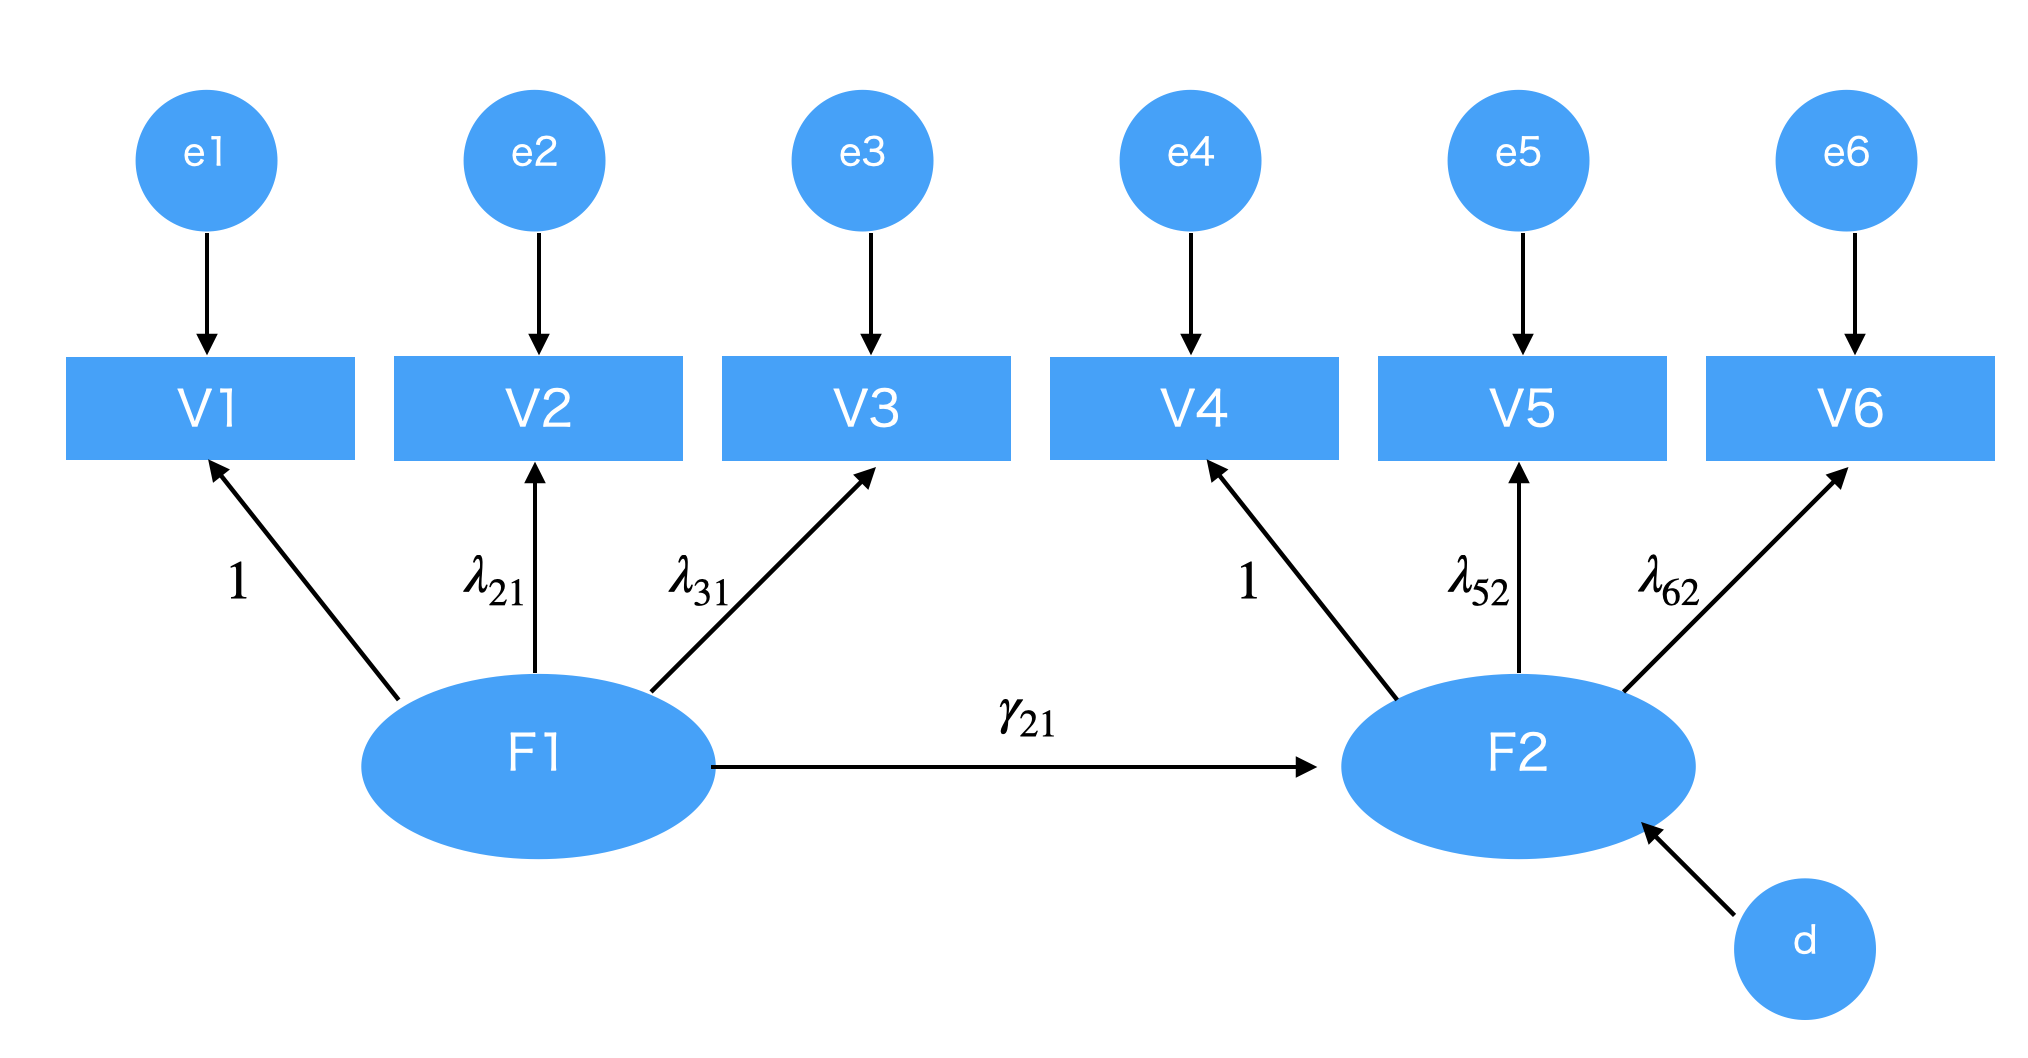
\includegraphics[width=0.8\linewidth,keepaspectratio]{../images/Slide12_05.png}
        \caption{構造方程式と測定方程式。記号の意味は後述}
        \label{fig::12_05}
    \end{center}
\end{figure}

ここで図\ref{fig::12_05}の係数について説明します。ギリシア文字$\lambda$や$\gamma$がパス係数を表しています。パス係数の添字は，被説明変数の変数番号$j$と，説明変数の変数番号$k$をつかって$\lambda_{jk}$のようにかき，これで$k \to j$の影響力の大きさを表していると思ってください。測定方程式の係数を$\lambda$で，構造方程式の係数を$\gamma$で表現しました。
% また$\lambda_{11},\lambda_{42}$になるべきところが$1$になっていますが，これは「潜在変数から出るパスのうち，1つは必ず$1$にしないと推定できない」という数学的特徴があるからです。決まりごとだと思ってください。

それを踏まえて，モデルの方程式を書くと，次のようになります。
\[ \left \{
    \begin{array}{rcl}
        V_1 & = & f_1 + e_1             \\
        V_2 & = & \lambda_{21}f_1 + e_2 \\
        V_3 & = & \lambda_{31}f_1 + e_3 \\
        V_4 & = & f_2 + e_4             \\
        V_5 & = & \lambda_{52}f_2 + e_5 \\
        V_6 & = & \lambda_{62}f_2 + e_6 \\
        f_2 & = & \gamma_{21}f_1 + d
    \end{array}
    \right .
\]
ややこしいだけで，書けるのは書けましたね。そして当然，これは行列表現した方が楽ではないか，というアイデアが浮かぶと思います。その通りで，エレメントワイズに書いてみましょう。

\[
    \begin{pmatrix} V_1 \\ V_2 \\ V_3 \\ V_4 \\ V_5 \\ V_6 \\ f_2 \\f_1 \end{pmatrix} =
    \begin{pmatrix} 0 & 0 & 0 & 0 & 0 & 0 & 0            & 1            \\
                0 & 0 & 0 & 0 & 0 & 0 & 0            & \lambda_{21} \\
                0 & 0 & 0 & 0 & 0 & 0 & 0            & \lambda_{31} \\
                0 & 0 & 0 & 0 & 0 & 0 & 1            & 0            \\
                0 & 0 & 0 & 0 & 0 & 0 & \lambda_{52} & 0            \\
                0 & 0 & 0 & 0 & 0 & 0 & \lambda_{62} & 0            \\
                0 & 0 & 0 & 0 & 0 & 0 & 0            & \gamma_{21}  \\
                0 & 0 & 0 & 0 & 0 & 0 & 0            & 0\end{pmatrix}
    \begin{pmatrix} V_1 \\ V_2 \\ V_3 \\ V_4 \\ V_5 \\ V_6 \\ f_2 \\f_1 \end{pmatrix} +
    \begin{pmatrix} e_1 \\ e_2 \\ e_3 \\ e_4 \\ e_5 \\ e_6 \\ d \\f_1 \end{pmatrix}
\]

左辺のベクトルの最後に$f_1$が入っているところがポイントで，これは方程式的には$f_1=f_1$というだけの式なのですが，これを入れたおかげで全体を整合的に表現できましたね。
この左辺のベクトルを$\bm{v}$として，式全体を$\bm{v} = \bm{Gv}+\bm{e}$と考えてみましょう。すると次のように展開できます。

\begin{eqnarray*}
    \bm{v} &=& \bm{Gv}+\bm{e}\\
    \bm{v}-\bm{Gv} &=& \bm{e}\\
    (\bm{I}-\bm{G})\bm{v} &=& \bm{e}\\
    (\bm{I}-\bm{G})^{-1}(\bm{I}-\bm{G})\bm{v} &=& (\bm{I}-\bm{G})^{-1}\bm{e}\\
\end{eqnarray*}
ここで$\bm{P} = (\bm{I}-\bm{G})$とすると，
\[ \bm{v} = \bm{P}^{-1}\bm{e} \]
ということになります。これをエレメントワイズで書くと次のようになります。
\[
    \begin{pmatrix} V_1 \\ V_2 \\ V_3 \\ V_4 \\ V_5 \\ V_6 \\ f_2 \\f_1 \end{pmatrix} =
    \begin{pmatrix} 1 & 0 & 0 & 0 & 0 & 0 & 0             & -1            \\
                0 & 1 & 0 & 0 & 0 & 0 & 0             & -\lambda_{21} \\
                0 & 0 & 1 & 0 & 0 & 0 & 0             & -\lambda_{31} \\
                0 & 0 & 0 & 1 & 0 & 0 & -1            & 0             \\
                0 & 0 & 0 & 0 & 1 & 0 & -\lambda_{52} & 0             \\
                0 & 0 & 0 & 0 & 0 & 1 & -\lambda_{62} & 0             \\
                0 & 0 & 0 & 0 & 0 & 0 & 1             & -\gamma_{21}  \\
                0 & 0 & 0 & 0 & 0 & 0 & 0             & 1\end{pmatrix}
    \begin{pmatrix} e_1 \\ e_2 \\ e_3 \\ e_4 \\ e_5 \\ e_6 \\ d \\f_1 \end{pmatrix}
\]

さて，変数からなるベクトル$\bm{v}$ではありますが，観測変数は$V_1$から$V_6$までしかありませんから，そこだけを取り出す行列$\bm{F}=\{ \bm{I},\bm{O} \}$を考えます。ここでは次のような行列です。
\[
    \bm{F} =
    \begin{pmatrix} 1 & 0 & 0 & 0 & 0 & 0 & 0 & 0 \\
                0 & 1 & 0 & 0 & 0 & 0 & 0 & 0 \\
                0 & 0 & 1 & 0 & 0 & 0 & 0 & 0 \\
                0 & 0 & 0 & 1 & 0 & 0 & 0 & 0 \\
                0 & 0 & 0 & 0 & 1 & 0 & 0 & 0 \\
                0 & 0 & 0 & 0 & 0 & 1 & 0 & 0\end{pmatrix}
\]
これを使って，次のように関係を書き直すことができます。
\[
    \bm{g} = \begin{pmatrix}  V_1 \\ V_2 \\ V_3 \\ V_4 \\ V_5 \\ V_6 \end{pmatrix} = \bm{FP^{-1}e}
\]
さて，ではデータだけのベクトル$\bm{g}$から分散共分散行列を構成するとしましょう。データベクトル$\bm{g}$は平均が0だと仮定します\footnote{ずいぶんと勝手な仮定だな，と思うかもしれませんが，分析の元になる変数ベクトルを標準化したと思っていただければそれほどおかしなことでもない，と考えてもらっても構いません。あるいは単に変数ごとの平均をとった平均偏差ベクトルを作って，それをデータだとしたと考えてください。}。そうすると分散共分散行列$\bm{\Sigma}$は次のようになります。

\begin{eqnarray*}
    \bm{\Sigma} &=& \bm{gg'}  \\
    & = & \bm{ F P^{-1} e ( F P^{-1} e) '} \\
    & = & \bm{ FP^{-1} ee' P^{-1'} F' }
\end{eqnarray*}

ここで式の中にある$\bm{ee'}$は誤差などの未知数で作った分散共分散行列になっています。誤差は他の変数との共分散がないと考えられるので，これは結局対角行列です。
\[
    \bm{ee'}= \begin{pmatrix}  V(e_1) &        &        &        &        &  &        &      &        \\
                        & V(e_2) &        &        &        &  &        &      &        \\
                        &        & V(e_3) &        &        &  &        &      &        \\
                        &        &        & V(e_4) &        &  &        &      &        \\
                        &        &        &        & V(e_5) &  &        &      &        \\
                        &        &        &        &        &  & V(e_6) &      &        \\
                        &        &        &        &        &  &        & V(d) &        \\
                        &        &        &        &        &  &        &      & V(f_1)\end{pmatrix}
\]

さあややこしい話はここまでにして，何を考えていたのかをもう一度考えてみましょう。

この式の左辺は$\bm{\Sigma}$，すなわちデータからできる分散共分散行列であり，具体的に数字の計算のできるデータセットです。この式の右辺は$\bm{ FP^{-1} ee' P^{-1'} F' } $であり，係数と潜在変数の分散からなる方程式です。左辺にデータ，右辺にモデルで表した分散共分散行列があり，これがイコールで結びついているのですから，この連立方程式を解けば，係数を求めることができます。

そりゃその計算はとても面倒なことになると思われますが，そこは機械がやってくれるのだ，と割り切ればいいでしょう。モデルがデータに最も合うように，未知数を決めていく方法は，\keytermL{最小二乗法}{さいしょうにじょうほう}や\keytermL{最尤法}{さいゆうほう}など，今まで学んできた手法を使えばよいのです！

こうして自由なモデリング技術とその解法を私たちは手に入れることができました。構造方程式モデリングとは，変数間関係を細かく作り込んでいき，分散共分散行列の隅々まで考え尽くす究極のモデル，ということの意味が伝わったでしょうか。


\end{document}